\documentclass[paper=a4, 12pt]{scrartcl}

\usepackage[utf8]{inputenc}
\usepackage[T1]{fontenc}
\usepackage[ngerman]{babel}
\usepackage{amsmath, amssymb}
\usepackage{siunitx}
\usepackage{graphicx}
\usepackage[colorlinks, allcolors=black, urlcolor=blue]{hyperref}
\usepackage[style=alphabetic]{biblatex}
\usepackage{pgf}
\usepackage{booktabs}

\addbibresource{bibliography.bib}

\begin{document}
	\tableofcontents

	\section{Theoretische Grundlagen}

\renewcommand{\V}[1]{\textbf{#1}}

\subsection{Klassischer Hall-Effekt}\label{sec:HallEffekt}

Bringt man einen stromführenden Leiter in ein äußeres Magnetfeld mit nicht zum Leiter paralleler Flussrichtung, so kann man senkrecht zur Stromrichtung eine Spannung (die \emph{Hall-Spannung}) messen. Dies bezeichnet man als \emph{Hall-Effekt}.
Dieser kann klassisch wie folgt erklärt werden:
Bewegen sich die Ladungsträger in einem Magnetfeld, das einen senkrechten Anteil zur Bewegungsrichtung hat, so wirkt auf die Ladungsträger (Ladung $q$, Geschwindigkeit $v$) eine nicht-verschwindende \emph{Lorentz-Kraft} senkrecht zum Strom und zum Magnetfeld (zumindest bei fehlenden äußeren elektrischen Feldern). Die dadurch hervorgerufene Ablenkung der Ladungsträger führt zur Ausbildung eines elektrischen Feldes, welches eine der ablenkenden Kraft entgegengerichtete Kraft erzeugt. Dieses \emph{Hall-Feld} baut sich solange auf, bis die daraus resultierende Kraft die des Magnetfeldes gerade kompensiert.
Es folgt die Bedingung an die Lorentz-Kraft
$$\V F_L = q(\V E_H + \V B\times \V v) = 0,$$
wobei $\V E_H$ das Hall-Feld bezeichne und $\V B$ senkrecht zum Strom sei.
Dadurch lassen sich die relevanten Größen in Beziehung setzen. Für die Hall-Spannung $U_H$ gilt bei einer Stromstärke $I$
\begin{equation}\label{eq:HallSpannung}
U_H\propto\frac{I\cdot B}{(\text{Probendicke}\parallel \V B)}.
\end{equation}
Die auftretende Proportionalitätskonstante wird \emph{Hall-Konstante} genannt und mit $A_H$ bezeichnet. Für diese gilt bei Leitung durch nur eine Sorte Ladungsträger
\begin{equation}
A_H = \frac{1}{nq}
\end{equation}
wobei $n$ die Ladungsträgerdichte (bzw. -konzentration) bezeichne. Diese kann also (bei
bekanntem $q$) durch Messung der Hall-Konstante bestimmt werden.
Anstatt $U_H$ lässt sich auch der \emph{Hall-Widerstand}
\begin{equation}\label{eq:HallWiderstand}
R_H = \frac{U_H}{I}
\end{equation}
betrachten, welcher zwar die Dimension eines Widerstands hat, jedoch nicht direkt mit einem „realen“ Widerstand identifiziert werden kann.\\
Gemessen werden jedoch stets $U_H$ und $I$.

\subsection{Zweidimensionales Elektronengas}
Um den \emph{Quanten-Hall-Effekt} beschreiben zu können, benötigt man das Modell des \emph{(2-dimensionalen) Elektronengases}\footnote{kurz: (2D)EG}.
Das EG ist ein Spezialfall des \emph{(idealen) Fermi-Gases}. Das ideale Fermi-Gas beschreibt passende Systeme durch ein Ensemble von nicht miteinander wechselwirkenden Fermionen in einem Potentialtopf, analog zum idealen Gas.
Angewandt auf die Elektronen im Festkörper bedeutet das also, dass neben den Wechselwirkungen der Elektronen miteinander auch das periodische Kristallpotential nicht wirklich berücksichtigt wird.\\

Dies kann aber zumindest teilweise durch das \emph{Bloch-Theorem} gerechtfertigt werden:\\
In einem periodischen Potential (endlicher Ausdehnung) erhält man eine Basis des Lösungsraumes bestehend aus Funktionen
$$\Psi_{\V k}(\V r) = u_{\V k}(\V r) e^{i\V k\cdot\V r},$$
wobei $\V k$ aus der ersten Brioullin-Zone stammt\footnote{Durch die Annahme endlicher Ausdehnung sind hier nur endlich viele $\V k$ möglich} und jedes $u_{\V k}$ dieselbe Periodizität wie das Potential hat.
Das periodische Potential der Kerne äußert sich also nur in einer Modulation\footnote{Störstellen können dieses Verhalten jedoch ändern} (\cite{czy15}, \cite{gro18}).\\

Speziell beim 2DEG nimmt man das Potential in einer Raumrichtung als Potentialtopf an. Für diese Richtung ergeben sich, wie für einen Potentialtopf üblich, (endlich viele) diskrete Energieniveaus. Die Menge der Lösungen der (stationären) eindimensionalen Schrödinger-Gleichung zu je einem dieser Energieeigenwerte bezeichnet man als \emph{Subband}.
In den anderen beiden Richtungen kann die Bewegung ungehindert ablaufen, wird also durch den Hamilton-Operator eines zweidimensionalen freien Teilchens beschrieben, jedoch mit einer effektiven Masse anstatt der üblichen Elektronenmasse.
Praktisch kann ein 2DEG z.B. an Grenzflächen passender Heterostrukturen erzeugt werden.

\subsection{Quanten-Hall-Effekt}\label{sec:Quanten-Hall-Effekt}
Führt man an einem 2DEG Versuche zum Hall-Effekt bei sehr niedrigen Temperaturen durch, so beobachtet man ein anderes Verhalten des Hall-Widerstands. Anstatt linear mit dem Magnetfeld anzuwachsen, bilden sich \emph{Hall-Plateaus} aus, die mit stärkerem Magnetfeld ausgeprägter werden. Beim Längswiderstand, also dem „realen“ Widerstand in Richtung des Stroms, kann man zudem die \emph{Shubnikov-de-Haas-Oszillationen} beobachten. Die Minima dieser Oszillation des Widerstands findet man bei denselben Feldstärken, wie die Hall-Plateaus. Für den Wert des Hall-Widerstands ergibt sich an diesen Stellen
\begin{equation}\label{eq:HallvKl}
R_H = \frac{1}{\nu}R_K
\end{equation}
wobei
\begin{equation}\label{eq:vKlitzing}
R_K := \frac{h}{e^2}
\end{equation}
als \emph{von-Klitzing-Konstante} bezeichnet wird und $\nu$ der sogenannte \emph{Füllfaktor} ist. Dieser nimmt zunächst ganzzahlige Werte an, die bei wachsenden Magentfeldern kleiner werden. Bei sehr hohen Magentfeldern erhält man jedoch auch echt rationale Werte für $\nu$. Man unterscheidet entsprechend den \emph{integralen} und den \emph{fraktionalen Quanten-Hall-
Effekt}.
Dem Füllfaktor lässt sich noch eine andere Bedeutung geben, welche auch die Namensgebung begründet.
In einem äußeren Magnetfeld wird die Bewegung der Elektronen auch in der „freien“ Ebene beeinflusst und entspricht dann nicht mehr der von freien Teilchen. Hat das Magnetfeld eine zur Ebene senkrechte Komponente, so lässt sich (klassisch) erklären, dass die Elektronen durch die Lorentz-Kraft auf Kreisbahnen gezwungen werden (vgl. \autoref{sc:HallEffekt}). Auf diesen bewegen sie sich mit der \emph{Zyklotronfrequenz}
$$\omega_C = \frac{eB}{m^*}$$
wobei das Magnetfeld $\V B$ wieder als senkrecht zur Ebene angenommen wurde und $m^*$ die effektive Masse bezeichne. Berechnet man nun die Energien, so erhält man neben den quantisierten Energien des Potentialtopfs und dem Beitrag der Spin-Magnetfeld-Wechselwirkung auch einen Beitrag durch Energieniveaus eines harmonischen Oszillators mit Frequenz $\omega_C$. Letztere werden auch als \emph{Landau-Niveaus} bezeichnet. Der Füllfaktor
lässt sich nun mit der Anzahl der besetzten Landau-Niveaus in Beziehung setzen. Man erhält dadurch letztlich
\begin{equation}\label{eq:Fuellfaktor}
\nu = \frac{n_eh}{Be}
\end{equation}
mit der Elektronenkonzentration $n_e$. Diese lässt sich also gemäß der Gleichung
\begin{equation}\label{eq:ElektrKonz1}
n_e = \frac{\nu Be}{h}
\end{equation}
aus einer Messung des Hall-Widerstands bestimmen, nachdem man die Plateaus den entsprechenden Füllfaktoren zugeordnet hat.
Alternativ kann man $U_H$, resp. $R_H$ auch gegen den Kehrwert $1/B$ des Magnetfeldes auftragen und die Periode
$\Delta$ bestimmen. $n_e$ ergibt sich dann gemäß
\begin{equation}\label{eq:ElektrKonz2}
n_e = \frac{2e}{h\Delta}.
\end{equation}
Für den klassischen Grenzfall $B\approx 0$ oder $T\gg0$ kann man (passend zu \eqref{eq:HallSpannung}-\eqref{eq:HallWiderstand}) auch
\begin{equation}\label{eq:ElektrKonz3}
n_e = \frac{1}{e}\left(\frac{\partial R_H}{\partial B}\right)^{-1}
\end{equation}
verwenden.\\
Die Elektronenmobilität ergibt sich zu
\begin{equation}\label{eq:Mobilitaet}
\mu_e \propto \frac{1}{e n_eR_{xx}(0)},
\end{equation}
wobei der Proportionalitätsfaktor durch das Verhältnis aus Kontaktabstand und Breite der Hallgeometrie gegeben ist.
\nocite{qhe}
\nocite{wiki-fg}
\nocite{wiki-he}

	\section{Aufbau und Durchführung}
Der erste Schritt bestand darin, das Programm zu schreiben, welches den Messvorgang steuert, also Magnetfeld hoch- und runterfährt, sowie Messwerte ausliest und in einer Datei speichert. Dazu wurde LabView verwendet.

\subsection{Magnetotransportmessung}\label{sec:Magnetotransport}
Bei diesen Messungen geht es darum, die Magnetotransporteigenschaften der Probe zu bestimmen.

\begin{wrapfigure}[13]{r}{7.5cm}

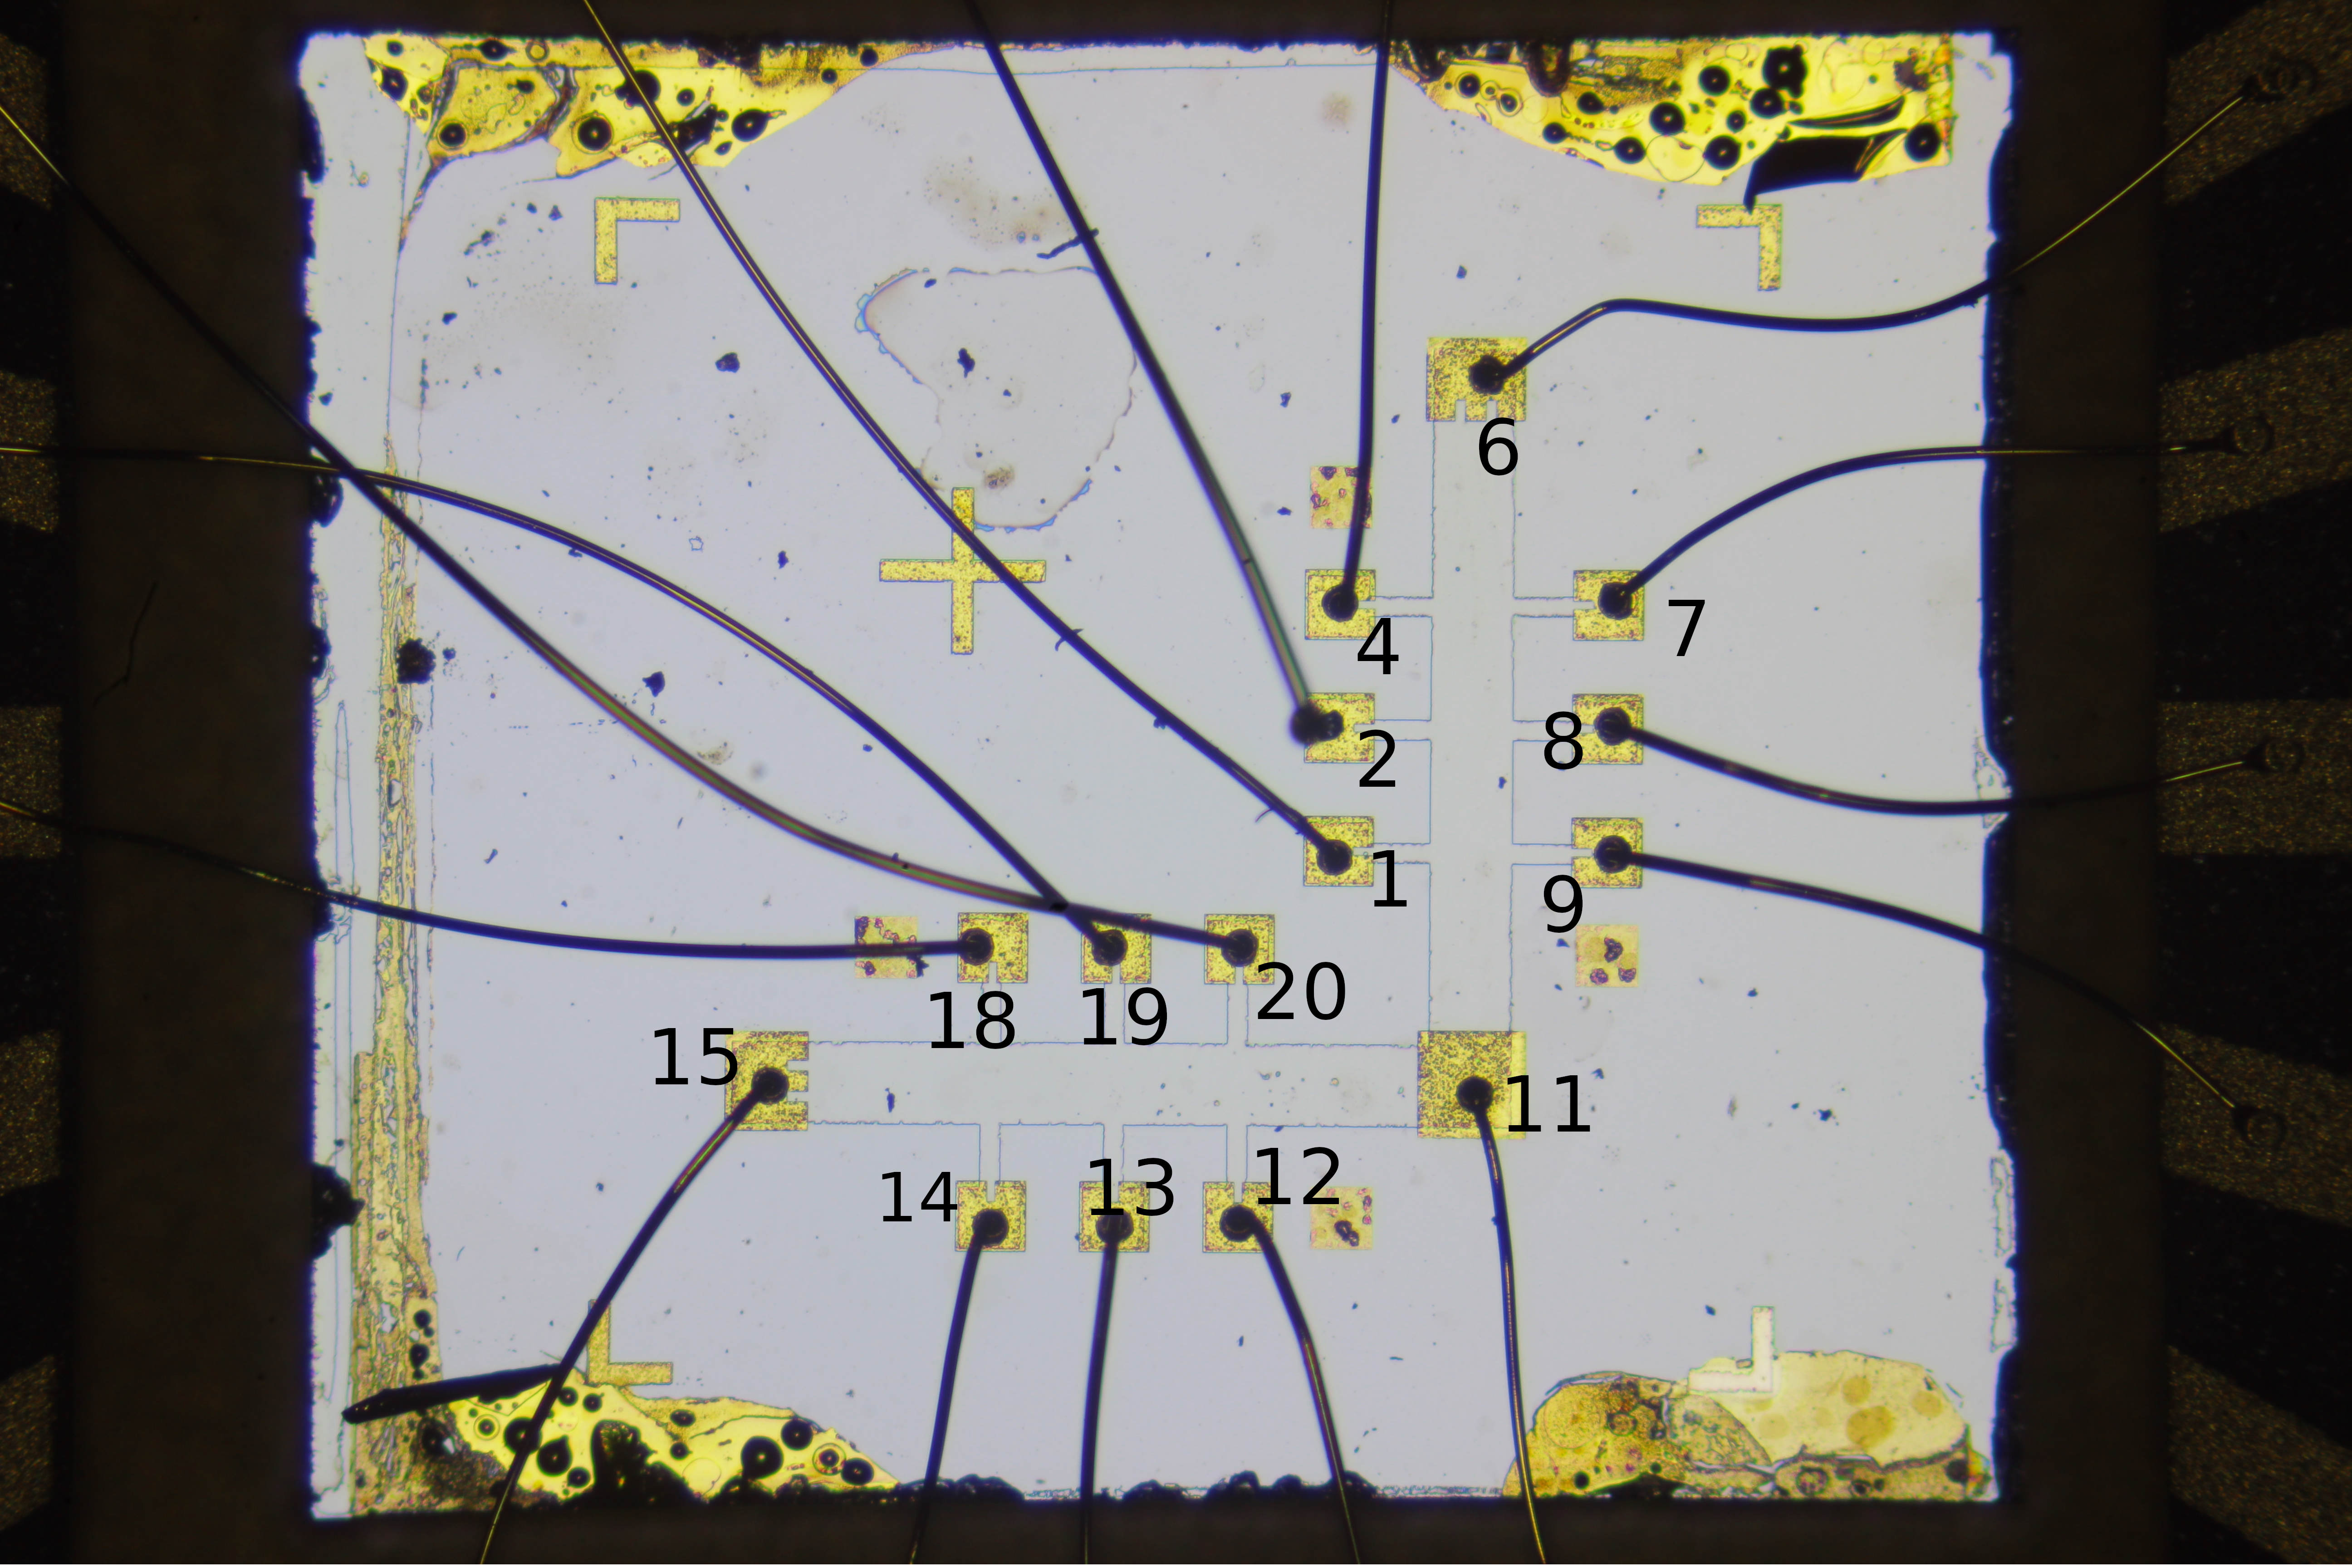
\includegraphics[scale=0.04]{Pictures/P07BondSchema.jpg}
\caption{Bond-Schema von Probe \emph{P07}}

\label{fig:P07}

\end{wrapfigure}
\hfill\\
Der Magnetprobenstab, an dessen unteren Ende sich eine Spule befindet, wird in der Heliumkanne platziert.
Die Probe (\emph{P07}, Bond-Schema siehe \autoref{fig:P07}) wird in den Probenstab eingesetzt und dieser wiederum in den Magnetprobenstab eingelassen.
Vor der ersten Messung muss lange genug gewartet werden, sodass die eingebrachten Bauteile abkühlen können.\\
Über ein Schaltbrett, das es erlaubt, auf die verschiedenen Kontakte der Hallgeometrie zuzugreifen, wird der Stab mit einer Stromquelle (\emph{Keithley 2400}) verbunden.
Zum Aufbauen des Magnetfelds wird ein weiteres Netzteil benötigt.
Mittels zweier \emph{Keithley 2000} werden Längs- und Querspannung gemessen.\\\\
Dabei wird der Längsstrom von $10\ \si{\micro A}$ an zwei verschiedene Kontaktpaare angelegt.
Für jedes Kontaktpaar werden die Spannungsmessgeräte wiederum mit jeweils zwei Kontaktpaaren verbunden, sodass vier Messreihen entstehen.
In jeder Messreihe wird das Magnetfeld von $0\ \si{T}$ auf $4\ \si{T}$ hochgefahren (oder andersherum) und in geeigneten Abständen werden Längs- und Querspannung aufgenommen.
Die Kontaktpaare sollen nach Möglichkeit verschieden sein, was jedoch aufgrund defekter Kontakte nicht immer uneingeschränkt möglich war.\\
Aus den Messwerten werden dann Elektronenkonzentration und -beweglichkeit bestimmt.\\\\
Die verwendeten Paarungen (inklusive den in \autoref{sec:Auswertung} verwendeten Bezeichnungen der Messreihen) sind in \autoref{tab:PairsP07} zu finden.\\

\begin{table}[ht]
\caption{Für die Messungen zum Magnetotransport verwendete Kontaktpaarungen}
\label{tab:PairsP07}
\centering
\begin{tabular}{cccc}
\toprule
Bezeichnung & Strom & Längswiderstand & Hallwiderstand\\
\midrule
P07\_1\_A & $6\rightarrow 11$ & $7\rightarrow 8$ & $1\rightarrow 9$\\
P07\_1\_B & $6\rightarrow 11$ & $7\rightarrow 9$ & $1\rightarrow 9$\\
P07\_2\_A & $11\rightarrow 15$ & $12\rightarrow 13$ & $20\rightarrow 12$\\
P07\_2\_B & $11\rightarrow 15$ & $20\rightarrow 18$ & $19\rightarrow 13$\\
\bottomrule
\end{tabular}
\end{table}
\subsection{Dauerhafter Photoeffekt}\label{sec:Photoeffekt}
Bei sehr tiefen Temperaturen kann der durch den Photoeffekt erzeugte Strom auch nach Ausschalten der Beleuchtung noch gemessen können.
Dies soll anhand dieser Messungen verifiziert werden.

\begin{wrapfigure}[13]{r}{7.5cm}
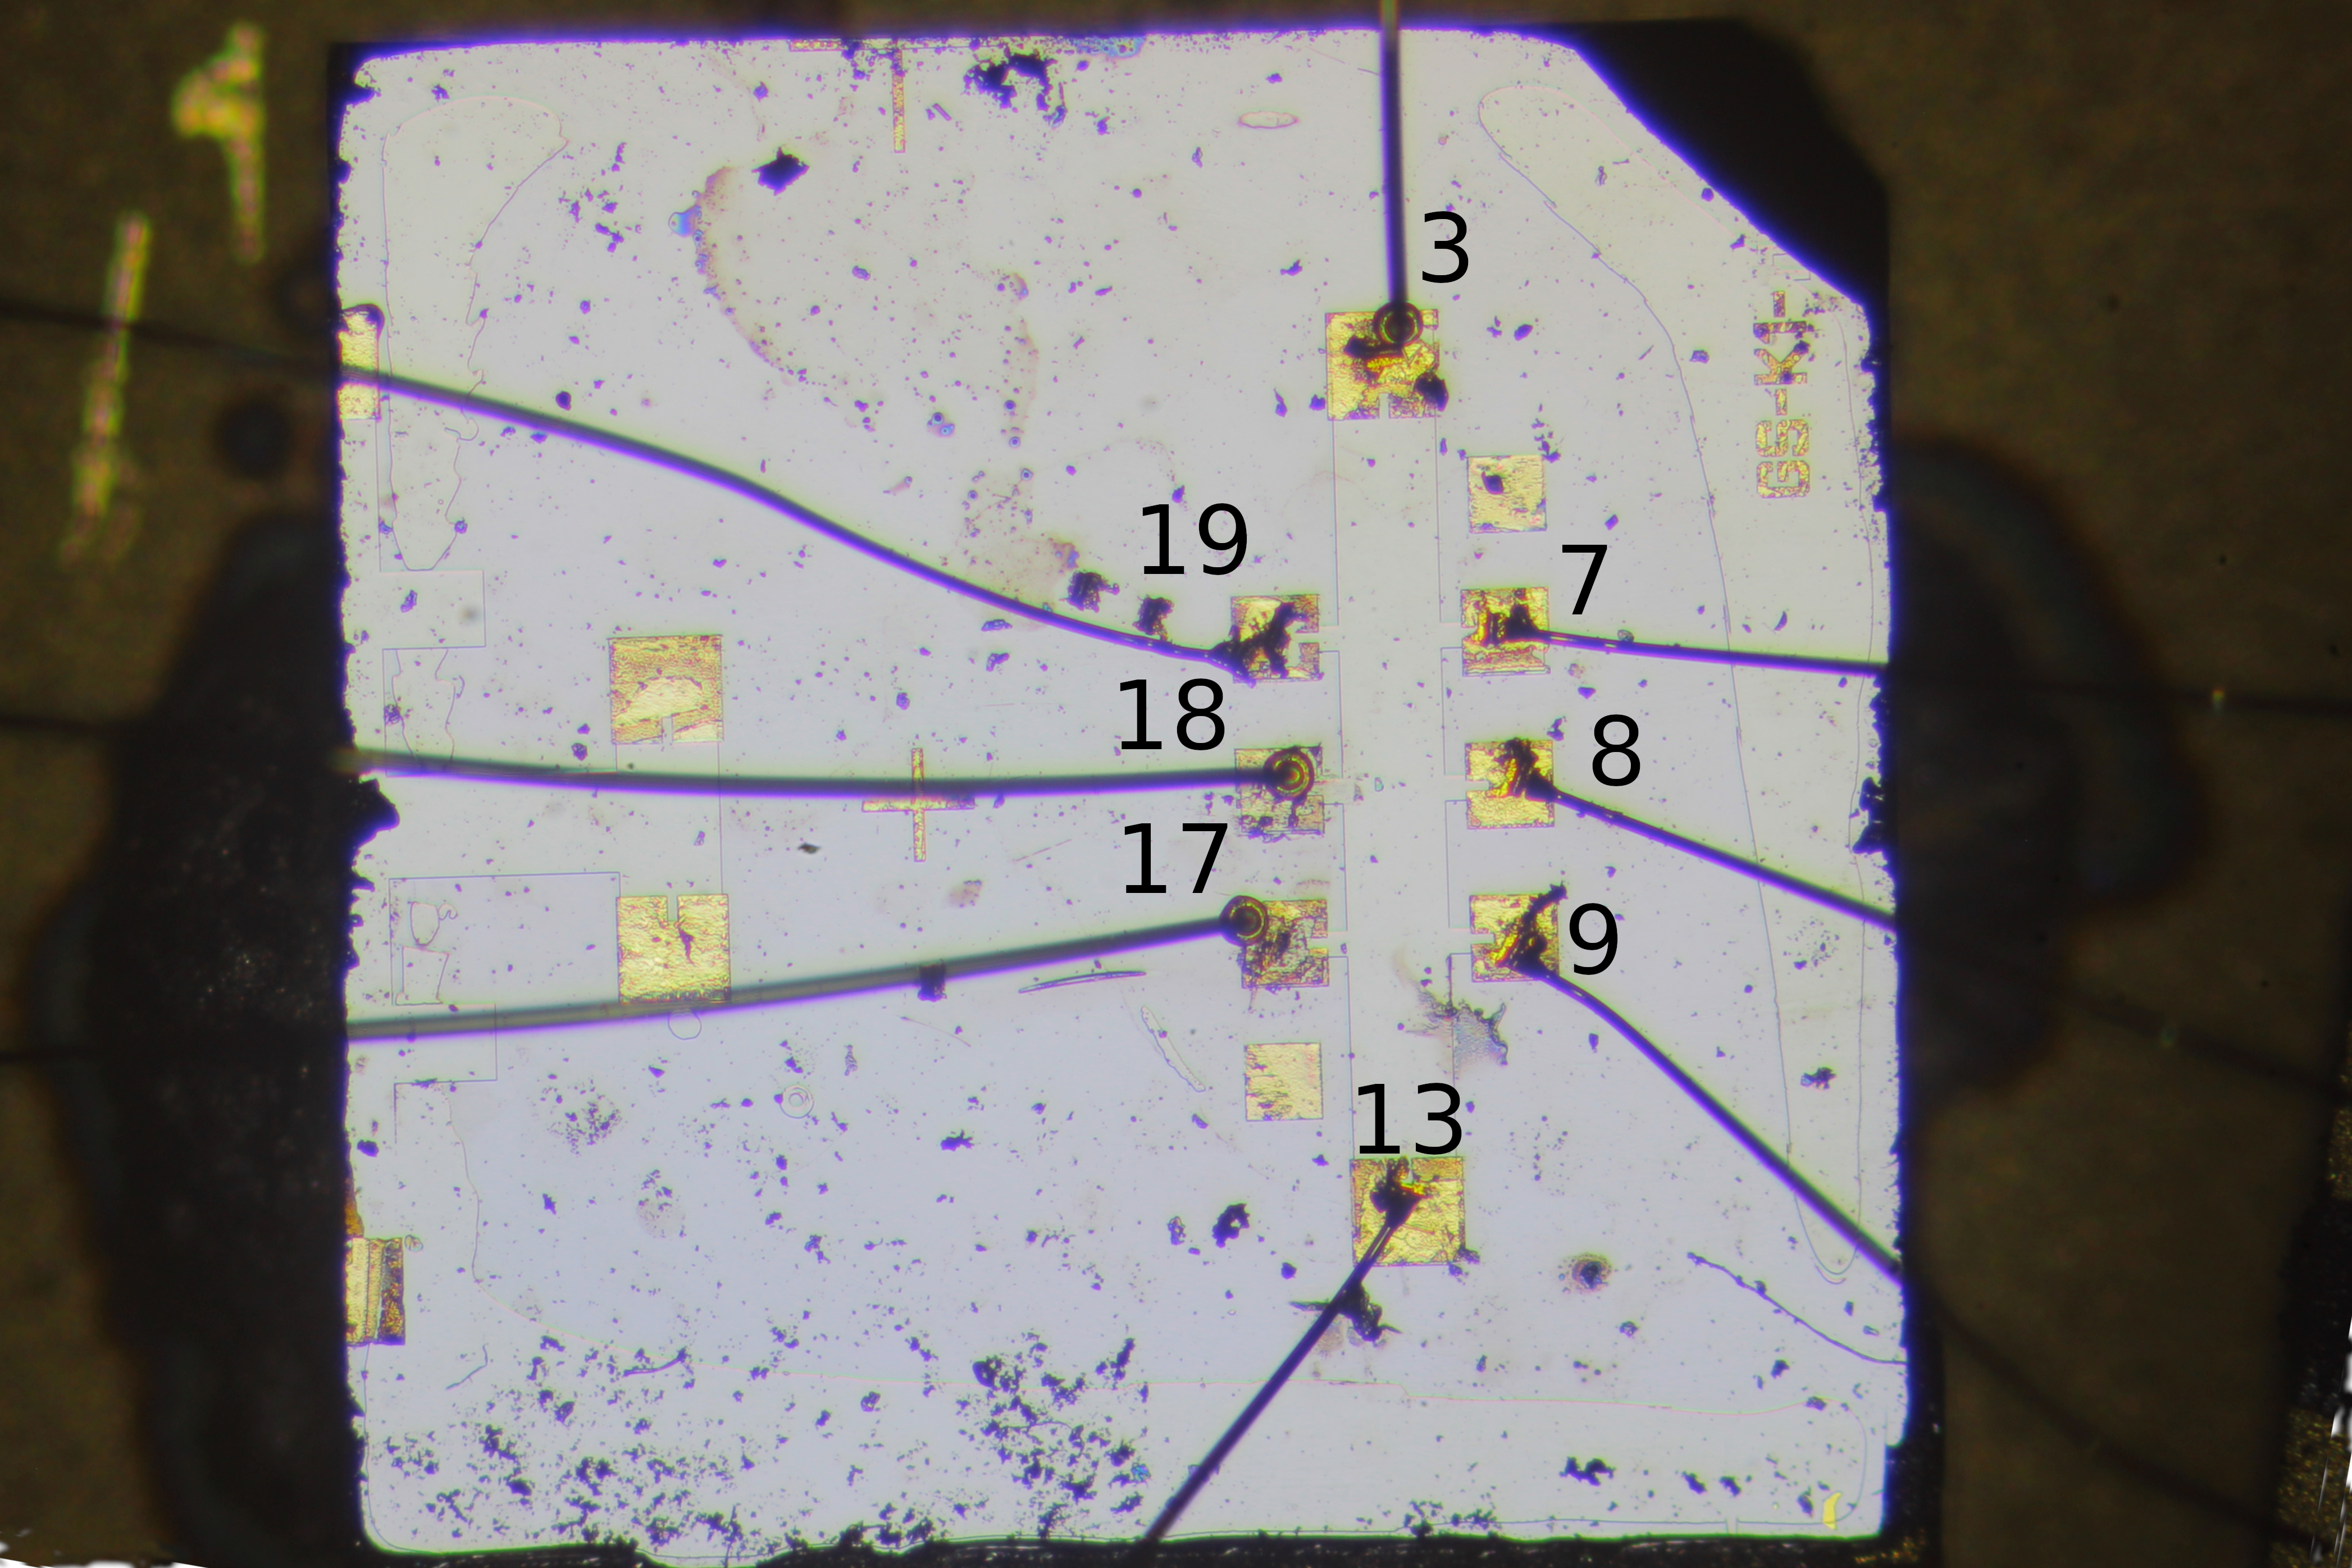
\includegraphics[scale=0.05]{Pictures/P04BondSchema}
\caption{Bond-Schema von Probe \emph{P04}}
\label{fig:P04}
\end{wrapfigure}
\hfill\\
Der Aufbau der Messung ist zum größten Teil identisch zu dem in \autoref{sec:Magnetotransport} beschriebenen. Es wird jedoch eine andere Probe (\emph{P04}, Bond-Schema siehe \autoref{fig:P04}) verwendet, auf welcher außerdem eine LED angebracht wird.

Bei diesen Messungen wird der Strom stets an dieselben Kontakte angelegt.
Zunächst werden für zwei Kombinationen von Kontakten Messungen analog zu \autoref{sec:Magnetotransport} durchgeführt. Die verwendeten Paarungen sind \autoref{tab:PairsP04} zu entnehmen.\\
Anschließend wird mit einem \emph{Keithley 2400} an die LED ein Strom von $8\ \si{mA}$ angelegt und die Probe für $60$ Sekunden beleuchtet.
Nach einer Wartezeit von zehn Minuten wird die Messung wiederholt.\\
Elektronenkonzentration und -beweglichkeit werden berechnet und verglichen.

\begin{table}[ht]
\caption{Für die Messungen zum Magnetotransport verwendete Kontaktpaarungen}
\label{tab:PairsP04}
\centering
\begin{tabular}{cccc}
\toprule
Bezeichnung & Strom & Längswiderstand & Hallwiderstand\\
\midrule
P04\_1 & $3\rightarrow 13$ & $7\rightarrow 8$ & $19\rightarrow 7$\\
P04\_2 & $3\rightarrow 13$ & $19\rightarrow 17$ & $17\rightarrow 9$\\
\bottomrule
\end{tabular}
\end{table}


	\printbibliography[heading=bibintoc]
\end{document}
